%20
\begin{frame}
  \small
  \begin{itemize}
    \item Bekezdések \texttt{<p>} elemmel jelölhetők
    \item Például: \texttt{<p title="Bek. 1">Első bekezdés.</p><p>Második bekezdés.</p>}
    \item \texttt{title} globális attribútum felugró szövegdoboz, ,,tooltip'' szöveg megadására
    \item Alapértelmezetten térközt hagy a böngésző a bekezdések között
    \item Sortörés új bekezdés (és térköz) nélkül: \texttt{<br />}
    \item Előformázott szöveg (pl. karakteres módú program kimenete), egyenszélességű (monospace) karakterekkel, forrás fehér karaktereinek megőrzésével: \texttt{<pre>}
  \end{itemize}
  \vfill
  ,,Tradicionális'' \hiv{\href{https://developer.mozilla.org/en-US/docs/Web/HTML/Block-level_elements}{tördelési módok}}
  \begin{description}[m]
    \item[Blokkszintű] (block) \hfill \\ Új sorban kezdődik, és a teljes elérhető szélességet elhasználja, pl. \texttt{<p>}, \texttt{<pre>}, \texttt{<h1>}-\texttt{<h6>}, \texttt{<hr />}
    \item[Soron belüli] (inline) \hfill \\ Aktuális sorban kezdődik, csak olyan széles helyet foglal, ahol éppen elfér, pl. \texttt{<br />}
  \end{description}
\end{frame}

%21
\begin{frame}
  \begin{columns}[c]
    \column{0.75\textwidth}
      Formázza meg a \textattachfile{attila.txt}{verset} a mellékelt ábra szerint, azaz
      \begin{itemize}
        \item a költő neve legyen első szintű címsor, 
        \item a mű címe második szintű,
        \item a szakaszok (arab számokkal jelölve) harmadik szintűek.
        \item A bekezdéseket és a bekezdésen belüli sortöreseket állítsa be!
        \item A bekezdések fölé mozgatva az egeret lássuk a bekezdés sorszámát, pl. 1/1, 1/2, \dots, 2/3
      \end{itemize}
    \column{0.25\textwidth}
      \begin{center}
        \begin{exampleblock}{\textattachfile{attila.html}{attila.html}}
          \centering 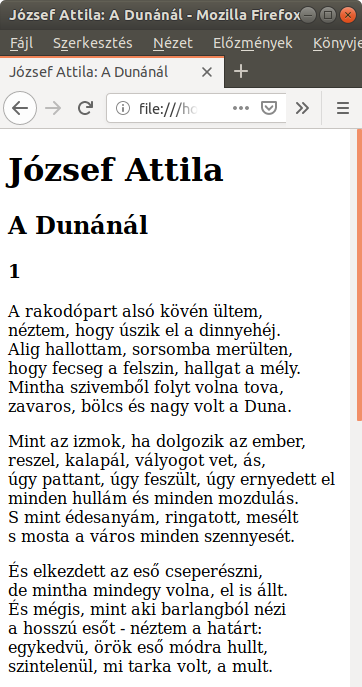
\includegraphics[scale=.2]{attila.png}
        \end{exampleblock}
      \end{center}
  \end{columns}
\end{frame}

%22
\begin{frame}
  \begin{columns}[c]
    \column{0.7\textwidth}
      Formázza meg a klasszikus Fahrenheit-Celsius átváltó 
      \textattachfile{fahrcels.c}{program} \textattachfile{fahrcels.txt}{kimenetét} 
      a mellékelt ábra szerint, azaz őrizze meg a program karakteres kimenetének formázását 
      a \texttt{<pre>} elemmel!
      
      A \texttt{<pre>} elem megőrzi a HTML forrásban lévő szóközöket, sortöréseket, és monospace betűtípust használ.
    \column{0.3\textwidth}
      \begin{center}
        \begin{exampleblock}{\textattachfile{fahrcels.html}{fahrcels.html}}
          \centering 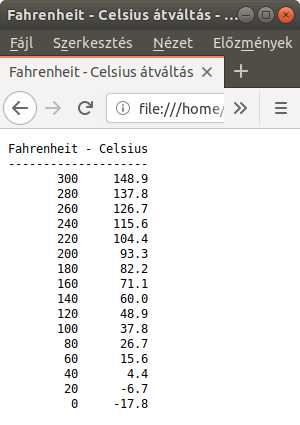
\includegraphics[scale=.35]{fahrcels.png}
        \end{exampleblock}
      \end{center}
  \end{columns}
\end{frame}
